\documentclass[conference]{IEEEtran}
\IEEEoverridecommandlockouts

\usepackage{cite}
\usepackage{amsmath,amssymb,amsfonts}
\usepackage{graphicx}
\usepackage{textcomp}
\usepackage{xcolor}
\usepackage{url}
\usepackage{balance}
\begin{document}

\title{Hybrid Model Predictive and Nonlinear Feedback Control for Chaos Suppression and MPPT Enhancement in DFIG-Based Wind Energy Systems}

\author{\IEEEauthorblockN{Said Regani}
\IEEEauthorblockA{\textit{L2EI Laboratory} \\
\textit{Jijel University}\\
BP 98 Ouled Aissa, Jijel 18000, Algeria}
\and
\IEEEauthorblockN{Manal Messadi}
\IEEEauthorblockA{\textit{L2EI Laboratory} \\
\textit{Jijel University}\\
BP 98 Ouled Aissa, Jijel 18000, Algeria}
\and
\IEEEauthorblockN{Karim Kemih}
\IEEEauthorblockA{\textit{L2EI Laboratory} \\
\textit{Jijel University}\\
BP 98 Ouled Aissa, Jijel 18000, Algeria}
}

\maketitle

\begin{abstract}
Doubly fed induction generator (DFIG)-based wind turbines are strongly nonlinear electromechanical systems that may exhibit irregular, and even chaotic, oscillations under abnormal operating conditions. This paper revisits the third-order rotor-current/speed model of the DFIG with a physically consistent parameter set, derives an equivalent dimensionless form, and shows by Lyapunov exponents and bifurcation analysis that chaotic motion appears only for strongly detuned mechanical damping and abnormal rotor excitation. A hybrid controller acting only on the rotor voltages is then proposed. An outer speed loop generates the torque-current reference, nonlinear feedback linearization cancels the coupled current dynamics, and a constrained, receding-horizon model predictive controller (MPC) with integral action handles the converter voltage limits; the MPC terminal weight and local gain are obtained from a linear matrix inequality (LMI) that guarantees nominal closed-loop stability. The controller is evaluated on chaos suppression and on maximum power point tracking (MPPT) of a 2-MW-class DFIG under turbulent wind and $\pm 20\,\%$ parameter mismatch, and compared with a feedback-linearization-only law and a PI law using the same gains. Using only the rotor voltages, with a cascaded speed loop, it suppresses chaos without steady-state error in all mismatch cases and settles 35--43\,\% faster than PI. It tracks the MPPT references with a speed error 5--140 times lower than PI and a power root-mean-square error of 0.6--1.7\,\% of rated power, three to eight times lower than with PI.
\end{abstract}

\begin{IEEEkeywords}
Doubly fed induction generator (DFIG), wind energy, chaotic dynamics, maximum power point tracking (MPPT), model predictive control (MPC), feedback linearization, linear matrix inequality (LMI).
\end{IEEEkeywords}

\section{Introduction}

Rising electricity demand and the depletion of fossil resources call for sustainable energy sources such as wind \cite{r1,r2,r3}. Wind power has grown rapidly \cite{r4}: a record 117~GW was installed in 2024, bringing the cumulative capacity to about 1136~GW \cite{r5}, driven by supportive policies and declining costs \cite{r6}.

The doubly fed induction generator (DFIG) dominates large onshore wind farms because its partial-scale back-to-back converter, rated at about 25--30\,\% of the generator power, allows decoupled control of active and reactive power over a wide speed range \cite{r7,r8,r9,r10,r11}. Its dynamic modelling, vector control and fault ride-through have been studied extensively \cite{r12,r13,r14,r15,r16}, and grid codes impose strict requirements on its dynamic behaviour \cite{r17,r18,r19}.

The electromechanical coupling between the rotor currents, the stator flux and the shaft speed makes the DFIG a strongly nonlinear system. Oscillatory transients \cite{r20} and, under particular parameter ranges or working conditions, chaotic behaviour have been reported \cite{r21,r22}; chaotic oscillations have also been analysed in other wind-turbine subsystems \cite{r23}. Chaos in electrical machines is usually analysed on dimensionless models \cite{r24,r25} and suppressed by nonlinear or adaptive feedback \cite{r24,r26,r27} or by predictive control \cite{r25,r28,r29,r30,r31}; robust sliding-mode and fault-tolerant controllers have also been proposed for wind turbines \cite{r32,r33}, and chaos synchronization has applications such as secure communications \cite{r34}. For MPPT, combining feedback linearization with MPC has proven effective \cite{r35}.

A critical point, often overlooked, is whether the parameters used to exhibit chaos are physically admissible. In this paper: (i) the DFIG model of \cite{r36} is written with a physically consistent parameter set ($L_s,L_r>L_m$, $0<\sigma<1$) and all constants of the state equations are given explicitly; (ii) a dimensionless form is derived, which shows that chaos requires strongly abnormal damping and rotor excitation, and the chaotic regime is characterized by Lyapunov exponents and a bifurcation diagram; (iii) a hybrid controller combining feedback linearization with a constrained MPC is designed, with an LMI-based terminal cost that guarantees nominal stability; (iv) quantitative comparisons with two baselines under parameter mismatch are reported for chaos suppression and for MPPT tracking.

\section{Wind Turbine Model}

The aerodynamic power captured by the rotor is \cite{r37,r32,r33}
\begin{equation}
P_{a} = \tfrac{1}{2}\rho\pi R^{2}C_{p}(\lambda)\, v^{3},\qquad \lambda = \frac{R\,\Omega_{t}}{v},
\label{eq1}
\end{equation}
where $\rho$ is the air density, $R$ the blade radius, $v$ the wind speed, $\Omega_t$ the turbine speed, and $C_p$ the power coefficient, maximal ($C_{p,\max}$) at $\lambda=\lambda_{opt}$. We use $C_p(\lambda)=0.5176(116/\lambda_i-5)e^{-21/\lambda_i}+0.0068\lambda$ with $1/\lambda_i=1/\lambda-0.035$ (zero pitch). Through a gearbox of ratio $G$, the generator mechanical speed is $\Omega_m=G\Omega_t$ and the electrical rotor speed is $\omega_r=n_p\Omega_m$, $n_p$ being the number of pole pairs. With the motor sign convention, the shaft dynamics referred to the generator side are
\begin{equation}
J\frac{d\Omega_{m}}{dt} = T_{e} - T_{L} - D\,\Omega_{m},\qquad T_L=-\frac{P_a}{\Omega_m},
\label{eq2}
\end{equation}
where $J$ is the total equivalent inertia, $D$ the viscous damping, and $T_e$ the electromagnetic torque ($T_e<0$ in generating mode). In the synchronous $dq$ frame, $T_{e} = \tfrac{3}{2}n_{p}( \psi_{ds}i_{qs} - \psi_{qs}i_{ds})$.

\section{DFIG Model and Chaotic Dynamics}

\subsection{Physically Consistent State Model}

The stator flux is aligned with the $q$ axis ($\psi_{qs}=\psi_s$, $\psi_{ds}=0$) and, neglecting the stator resistance in the flux relation, $u_{ds}=-V_s$, $u_{qs}=0$, $\psi_s=V_s/\omega_s$, where $V_s$ is the stator-voltage amplitude and $\omega_s$ the grid angular frequency. Then $i_{ds}=-(L_m/L_s)i_{dr}$ and $T_e=\tfrac{3}{2}n_p(L_m/L_s)\psi_s i_{dr}$. With $x=[x_1,x_2,x_3]^T=[i_{dr},i_{qr},\omega_r]^T$, the DFIG dynamics \cite{r36} read
\begin{equation}
\left\{ \begin{aligned}
\dot{x}_{1} &= a_{1}x_{1} + ( \omega_{s} - x_{3})x_{2} + a_{2}x_{3} + c_1 + u_1, \\
\dot{x}_{2} &= - ( \omega_{s} - x_{3})x_{1} + a_{1}x_{2} + c_2 + u_2, \\
\dot{x}_{3} &= a_{6}x_{1} - a_{7}x_{3} - a_{8},
\end{aligned} \right.
\label{eq3}
\end{equation}
with $\sigma = 1-L_m^2/(L_sL_r)$ and
\begin{equation}
\begin{gathered}
a_{1} = - \frac{R_{s}L_{m}^{2}}{\sigma L_{s}^{2}L_{r}} - \frac{R_{r}}{\sigma L_{r}},\quad a_{2} = - \frac{L_{m}\psi_{s}}{\sigma L_{r}L_{s}},\\
a_{3} = - \frac{L_{m}}{\sigma L_{s}L_{r}},\quad a_{4} = \frac{1}{\sigma L_{r}},\quad a_{5} = \frac{R_{s}L_{m}\psi_{s}}{\sigma L_{s}^{2}L_{r}},\\
a_{6} = \frac{3n_{p}^{2}L_{m}\psi_{s}}{2JL_{s}},\quad a_{7} = \frac{D}{J},\quad a_{8} = \frac{n_{p}}{J}T_{L},\\
c_1 = a_3u_{ds}+a_4u_{dr}^0,\quad c_2 = a_5 + a_3u_{qs}+a_4u_{qr}^0 .
\end{gathered}
\label{eq4}
\end{equation}
Here $u_{dr}^0,u_{qr}^0$ are constant (open-loop) rotor voltages and $u_{1,2}=a_4\Delta u_{dr,qr}$ are the control actions of the rotor-side converter, which are the only available inputs: the speed equation has no actuator and is governed through the electromagnetic torque, i.e., through $i_{dr}$. Without control, $u_1=u_2=0$.

Table~\ref{tab1} lists the nominal parameters of a representative 2-MW-class DFIG (stator-referred). They satisfy $L_s,L_r>L_m$ and $\sigma=0.0661\in(0,1)$. The resulting coefficients are $a_1=-31.14$~s$^{-1}$, $a_2=-1.013\times10^{4}$~A/rad, $a_3=-5.649\times10^{3}$ and $a_4=5.845\times10^{3}$~A/(V$\cdot$s), $a_5=1.018\times10^{4}$~A/s, $a_6=8.19\times10^{-2}$~rad/(A$\cdot$s$^2$) and $a_7=7.87\times10^{-6}$~s$^{-1}$. Because $u_{ds}=-\omega_s\psi_s$, $c_1+a_2\omega_s=a_4u_{dr}^0$: the constant $a_3u_{ds}=3.18\times10^{6}$~A/s exactly compensates $a_2\omega_s$, and $c_2=1.018\times10^4+a_4u_{qr}^0$~A/s. Every constant of \eqref{eq3} is therefore obtained from Table~\ref{tab1}.

\begin{table}[htbp]
\caption{Nominal Parameters (2-MW-Class DFIG and Turbine)}
\begin{center}
\begin{tabular}{|c|c||c|c|}
\hline
\textbf{Param.} & \textbf{Value} & \textbf{Param.} & \textbf{Value} \\
\hline
$R_{s}$ & $2.6$~m$\Omega$ & $n_p$ & $2$ \\
$R_{r}$ & $2.9$~m$\Omega$ & $V_s$ (line, rms) & $690$~V, $50$~Hz \\
$L_{m}$ & $2.5$~mH & $\psi_s$ & $1.793$~Wb \\
$L_{s}=L_r$ & $2.587$~mH & $J$ & $127$~kg$\cdot$m$^2$ \\
$\sigma$ & $0.0661$ & $D$ & $10^{-3}$~N$\cdot$m$\cdot$s/rad \\
$\tau=-1/a_1$ & $32.1$~ms & $R$, $G$ & $40$~m, $80$ \\
$\rho$ & $1.225$~kg/m$^3$ & $\lambda_{opt}$, $C_{p,\max}$ & $8.1$, $0.48$ \\
\hline
\end{tabular}
\label{tab1}
\end{center}
\end{table}

\subsection{Dimensionless Model and Conditions for Chaos}

Let $\tau=-1/a_1$, $\tilde t=t/\tau$, $k=a_7/(\tau a_6)$, and $z_1=x_1/k$, $z_2=x_2/k$, $z_3=\tau(x_3-\omega_s)$ (normalized slip speed). Then \eqref{eq3} with $u=0$ becomes
\begin{equation}
\left\{ \begin{aligned}
z_1' &= -z_1 - z_3z_2 + \gamma z_3 + \varepsilon_1,\\
z_2' &= -z_2 + z_3z_1 + \varepsilon_2,\\
z_3' &= s\,(z_1 - z_3) + \varepsilon_3,
\end{aligned}\right.
\label{eq5}
\end{equation}
where $(\cdot)'=d/d\tilde t$, $s=\tau D/J$, $\varepsilon_1=\tau(c_1+a_2\omega_s)/k$, $\varepsilon_2=\tau c_2/k$, $\varepsilon_3=-\tau^2(a_7\omega_s+a_8)$, and
\begin{equation}
\gamma = \frac{a_2a_6\tau}{a_7} = -\frac{3n_p^2L_m^2\psi_s^2\,\tau}{2\sigma L_rL_s^2D} < 0 .
\label{eq6}
\end{equation}
With physical parameters ($\sigma>0$), $\gamma$ is always negative. The divergence of \eqref{eq5} is $-(2+s)<0$, so the system is dissipative.

For the nominal machine, $s=2.5\times10^{-7}$ and the equilibrium is stable. Chaos appears only far from nominal. For $\gamma=-1$, $s=8$, $\varepsilon_1=\varepsilon_3=0$ and $\varepsilon_2=-85$, the Lyapunov spectrum, computed with the QR-based variational method \cite{r38} over 500 time units, is $(1.416,\,0.003,\,-11.419)$. Its sum equals the divergence $-10$, and the Kaplan--Yorke dimension is $2.12$. Fig.~\ref{fig1}(a)--(b) shows the resulting double-scroll attractor. The bifurcation diagram and the largest Lyapunov exponent versus $\varepsilon_2$ (Fig.~\ref{fig1}(c)--(d)) show a stable equilibrium for $\varepsilon_2>-15$ and chaos for $\varepsilon_2<-15$, interrupted by periodic windows near $\varepsilon_2\approx-50.5$, $-41.8$ and $-28.5$.

Mapped back to Table~\ref{tab1}, this chaotic set requires $D/J\approx 250$~s$^{-1}$ (e.g., $J\approx13.6$~kg$\cdot$m$^2$ and $D\approx3.4$~kN$\cdot$m$\cdot$s/rad) and a $q$-axis rotor voltage of several kilovolts. Chaos is therefore not a feature of normal operation of this machine but a severe fault/detuning scenario, for which the controller must still guarantee recovery. Following common practice \cite{r24,r25}, chaos suppression is studied on \eqref{eq5}, whereas MPPT tracking is studied in physical units.

\begin{figure}[htbp]
\centerline{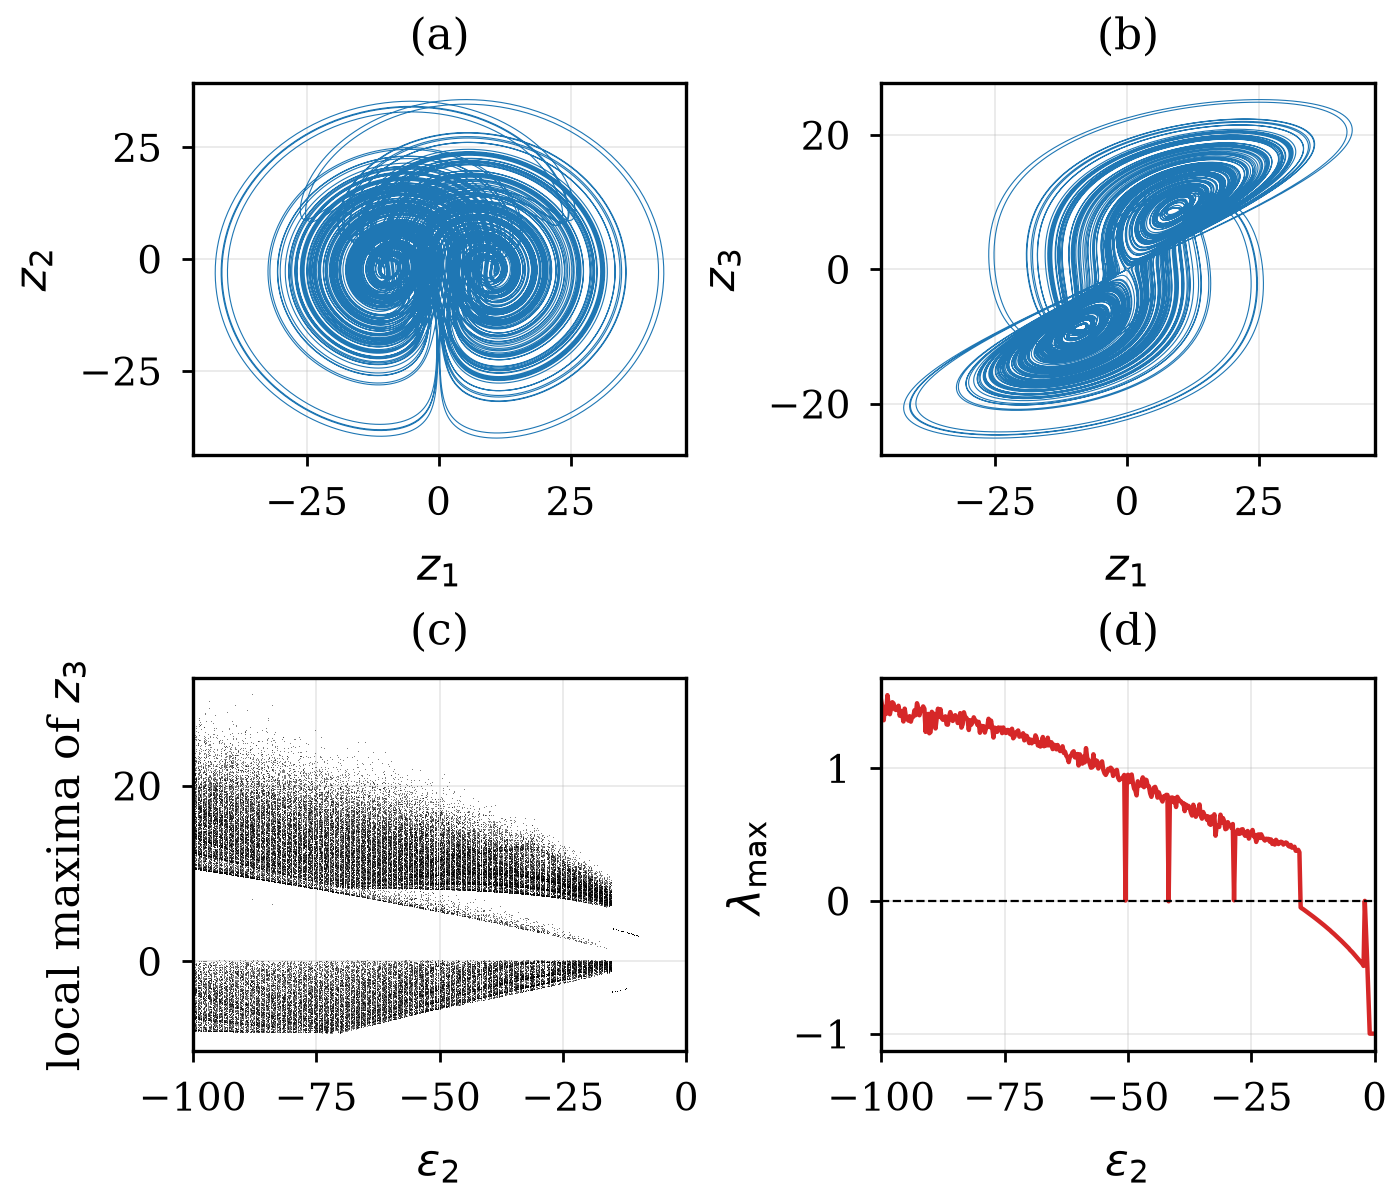
\includegraphics[width=0.48\textwidth]{fig1.png}}
\caption{Chaotic dynamics of \eqref{eq5} ($\gamma=-1$, $s=8$, $\varepsilon_1=\varepsilon_3=0$): (a) $z_1$--$z_2$ and (b) $z_1$--$z_3$ projections for $\varepsilon_2=-85$; (c) bifurcation diagram (local maxima of $z_3$) and (d) largest Lyapunov exponent versus $\varepsilon_2$.}
\label{fig1}
\end{figure}

\section{MPPT Reference Generation}

The wind speed is modelled as a mean value, three low-frequency harmonics and a smoothed Gaussian turbulence $v_{turb}$ (first-order filter, time constant 0.5~s):
\begin{equation}
v(t) = V_{mean} + \textstyle\sum_{k = 1}^{3}A_{k}\sin( 2\pi f_{k}t+\phi_k ) + v_{turb}(t),
\label{eq7}
\end{equation}
with $V_{mean}=9$~m/s, $(A_k)=(1.3,0.7,0.4)$~m/s and $(f_k)=(0.05,0.13,0.31)$~Hz (Fig.~\ref{fig2}).

\begin{figure}[htbp]
\centerline{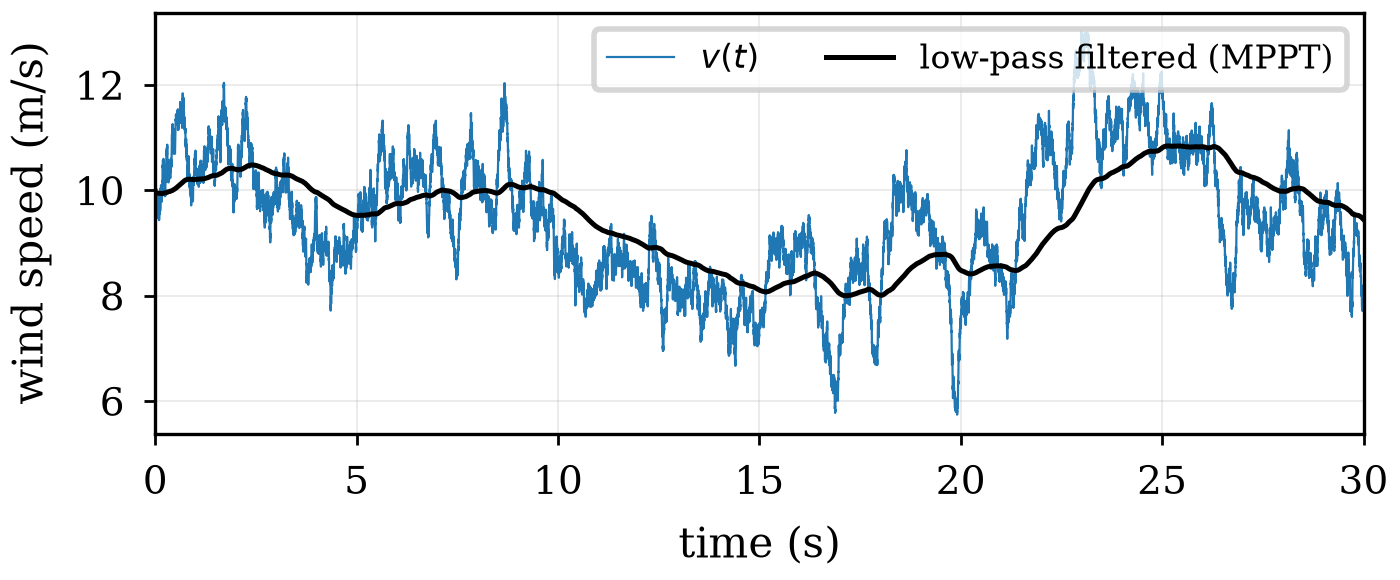
\includegraphics[width=0.48\textwidth]{fig2.png}}
\caption{Turbulent wind-speed profile and its low-pass filtered version used by the MPPT.}
\label{fig2}
\end{figure}

The optimal speed follows the low-pass filtered wind $\bar v$ (time constant 2~s):
\begin{equation}
\omega_{r,ref}(t) = n_pG\lambda_{opt}\,\bar v(t)/R .
\label{eq8}
\end{equation}
Since $T_e\propto i_{dr}$, the $d$-axis current reference is obtained from the torque balance of \eqref{eq3}, so that it is consistent with $\omega_{r,ref}$:
\begin{equation}
i_{dr,ref} = \frac{\dot\omega_{r,ref} + a_7\,\omega_{r,ref} + (n_p/J)\,T_L(v,\omega_{r,ref})}{a_6}.
\label{eq9}
\end{equation}
The stator reactive power is $Q_s=\tfrac32V_s i_{qs}=\tfrac32V_s(\psi_s-L_mi_{qr})/L_s$, so unity power factor ($Q_s=0$) gives
\begin{equation}
i_{qr,ref}=\psi_s/L_m .
\label{eq10}
\end{equation}
The generated stator active power and its reference are
\begin{equation}
P_s = -\tfrac32 V_s\frac{L_m}{L_s}\,i_{dr},\qquad P_{s,ref} = -\tfrac32 V_s\frac{L_m}{L_s}\,i_{dr,ref}.
\label{eq11}
\end{equation}
The reference trajectory is $x_d=[i_{dr,ref},\,i_{qr,ref},\,\omega_{r,ref}]^T$ and the tracking error is $e=x-x_d$.

\section{Hybrid Feedback-Linearization/MPC Design}

\subsection{Outer Speed Loop}

Since $T_e\propto i_{dr}$, the speed is controlled through the reference of $i_{dr}$ (cascade structure). With $e_\omega=\omega_r-\omega_{r,ref}$ and the nominal model,
\begin{equation}
i^\ast_{dr}=\frac{\dot\omega_{r,ref}+a_7\omega_r+\hat a_8(v,\omega_r)-\lambda e_\omega-\lambda_I\!\int\! e_\omega dt}{a_6},
\label{eqspd}
\end{equation}
which reduces to \eqref{eq9} when $e_\omega=0$. Substituting into the third line of \eqref{eq3} gives
\[
\dot e_\omega=-\lambda e_\omega-\lambda_I\!\int\! e_\omega dt+a_6\,(i_{dr}-i^\ast_{dr}).
\]
This is an exponentially stable linear system (poles: roots of $p^2+\lambda p+\lambda_I$) driven by the inner tracking error. It is therefore input-to-state stable, and $e_\omega\to0$ once $i_{dr}\to i^\ast_{dr}$ (cascade argument). The inner reference is $x_d=[i^\ast_{dr},\,i_{qr,ref}]^T$, and $\dot x_d$ is computed analytically from \eqref{eq3} and \eqref{eqspd}.

\subsection{Inner Loop: Feedback Linearization}

Write the first two lines of \eqref{eq3} as $\dot x_{1,2}=F_{1,2}(x,t)+u_{1,2}$ and let $\hat F_{1,2}$ be their nominal model. The control law
\begin{equation}
u_{1,2} = -\hat F_{1,2}(x,t) + \dot x_d + v
\label{eq12}
\end{equation}
gives the error dynamics $\dot e = v + \Delta(x,t)$, $e=[i_{dr}-i^\ast_{dr},\,i_{qr}-i_{qr,ref}]^T$, with $\Delta=F_{1,2}-\hat F_{1,2}$ ($\Delta=0$ nominally). This cancels the bilinear couplings $(\omega_s-x_3)x_{1,2}$ responsible for chaos, and leaves two decoupled integrators driven by the new input $v$.

\subsection{Constrained MPC with Integral Action}

For each channel $i$, the error is augmented with its integral, $\xi_i=[e_i,\ \int e_i\,dt]^T$, to remove steady-state errors due to $\Delta$. Sampling with period $T_s$ gives
\begin{equation}
\xi_i(k+1) = A\,\xi_i(k) + B\,v_i(k),\ \ A=\begin{bmatrix}1&0\\T_s&1\end{bmatrix}\!,\ B=\begin{bmatrix}T_s\\T_s^2/2\end{bmatrix}\!.
\label{eq13}
\end{equation}
At each instant $k$, the MPC solves the quadratic program
\begin{equation}
\begin{aligned}
\min_{v_i(\cdot|k)}\ & \sum_{j=1}^{N}\|\xi_i(k+j|k)\|_Q^2 + \|\xi_i(k+N|k)\|_P^2\\
& + r\sum_{j=0}^{N-1} v_i(k+j|k)^2\\
\text{s.t. }\ & \eqref{eq13},\qquad \underline v_i(k)\le v_i(k+j|k)\le \overline v_i(k),
\end{aligned}
\label{eq14}
\end{equation}
where $Q=Q^T>0$, $r>0$, and the input bounds $\underline v_i=-\bar u_i-h_i$, $\overline v_i=\bar u_i-h_i$, with $h=-\hat F+\dot x_d$, enforce the actuator limit $|u_i|\le\bar u_i$ on \eqref{eq12}. Only the first optimal move is applied (receding horizon). The integral state is frozen when the limit is reached (conditional integration).

\textit{Theorem 1:} Let $X=X^T>0$ and $Y$ satisfy the LMI
\begin{equation}
\begin{bmatrix}
X & (AX+BY)^T & XQ^{1/2} & \sqrt r\,Y^T\\
AX+BY & X & 0 & 0\\
Q^{1/2}X & 0 & I & 0\\
\sqrt r\,Y & 0 & 0 & 1
\end{bmatrix}\succeq 0,
\label{eq15}
\end{equation}
and set $P=X^{-1}$, $K=YX^{-1}$. Then
\begin{equation}
(A+BK)^TP(A+BK)-P+Q+rK^TK\preceq 0 .
\label{eq16}
\end{equation}
Let $\Omega=\{\xi:\xi^TP\xi\le\alpha\}$, with $\alpha>0$ small enough that $K\xi$ satisfies the input bounds in $\Omega$. If $\Delta=0$ and \eqref{eq14}, augmented with the terminal constraint $\xi_i(k+N|k)\in\Omega$, is feasible at $k=0$, then it remains feasible for all $k$ and $\xi_i=0$ is asymptotically stable, i.e., $x_{1,2}\to x_d$ and, with the outer loop, $\omega_r\to\omega_{r,ref}$.

\textit{Proof:} Applying the Schur complement to \eqref{eq15} with respect to its last three block rows gives $X-(AX+BY)^TX^{-1}(AX+BY)-XQX-rY^TY\succeq0$. Pre- and post-multiplying by $P=X^{-1}$ and substituting $Y=KX$ yields \eqref{eq16}. Hence $\Omega$ is positively invariant under $v=K\xi$, and $\xi^TP\xi$ is a control Lyapunov function in $\Omega$. By the standard terminal-cost/terminal-set argument \cite{r39}, the optimal cost $V_N^\ast$ of \eqref{eq14} then satisfies $V_N^\ast(k+1)-V_N^\ast(k)\le-\|\xi_i(k)\|_Q^2-r\,v_i(k)^2$ and the shifted solution completed by $K\xi$ is feasible, which proves recursive feasibility and asymptotic stability. \hfill$\blacksquare$

\textit{Remarks:} (i) The maximal-volume solution of \eqref{eq15} satisfies \eqref{eq16} with equality, i.e., $P$ is the solution of the discrete algebraic Riccati equation \cite{r40}. Consequently, when no constraint is active, \eqref{eq14} returns exactly $v_i=K\xi_i$. A single gain $K=[k_e,\,k_I]$, common to the two channels, is therefore obtained from the LMI and used in the implementation. (ii) Setting $k_I=0$ and ignoring constraints recovers the pure feedback-linearization law $v=-k_e e$ (``FL only''). Removing all model terms gives the classical cascaded PI vector control: a speed PI $i^\ast_{dr}=-(\lambda e_\omega+\lambda_I\!\int\! e_\omega)/a_6$ and current PIs $v=K\xi$. These two baselines use the same gains as the proposed controller, so the comparison isolates the effect of feedback linearization and of constrained MPC. (iii) The terminal constraint is not imposed explicitly in the simulations; convergence was verified a posteriori.

\begin{figure}[htbp]
\centerline{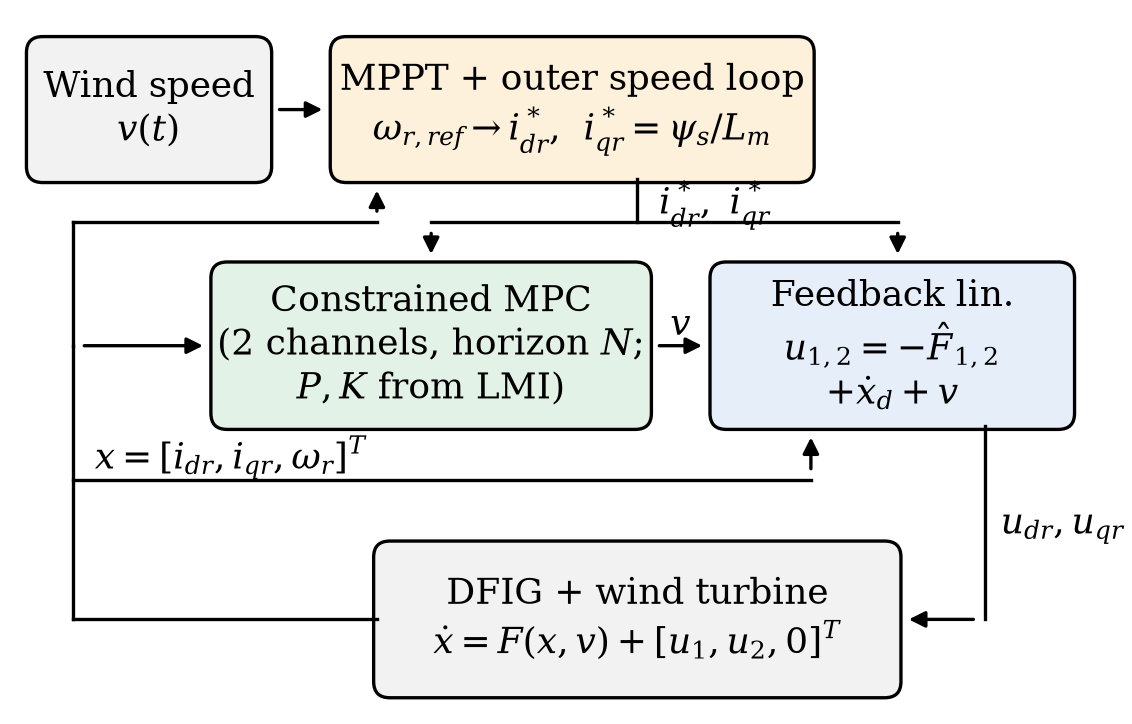
\includegraphics[width=0.46\textwidth]{fig3.png}}
\caption{Proposed cascaded architecture: outer speed loop, inner feedback-linearization/MPC current loops acting on the rotor voltages.}
\label{fig3}
\end{figure}

The overall structure is shown in Fig.~\ref{fig3}. The QP \eqref{eq14} has only $N$ variables per channel and was solved by a bounded-variable least-squares method.

\section{Simulation Results}

All simulations integrate the plant with a fourth-order Runge--Kutta scheme (4--5 sub-steps per sampling period). The controller uses the nominal model; the plant uses the nominal or perturbed parameters.

\subsection{Chaos Suppression}

System \eqref{eq5} is started in the chaotic regime and the controller is switched on at $\tilde t_{on}=6$ with $T_s=0.01$, $N=15$, $Q=\text{diag}(1,10)$, $r=10^{-4}$ and $|u_{1,2}|\le120$ (no input on the speed equation). The LMI gives $K=[-63.9,\,-192.4]$, and the outer loop on $z_3$ uses $\lambda=10$, $\lambda_I=25$ (double pole at $-5$). The target $z^\ast=(2.02,\,-2.00,\,2.02)$ corresponds to $\omega_r=1.2\,\omega_s$ (super-synchronous operation with positive speed). It is an equilibrium with $u_1^\ast=0$, sustained by $u_2^\ast=78.9$ alone, which compensates the abnormal excitation $\varepsilon_2$. Robustness is tested by scaling all coefficients of the plant by $0.8$ and $1.2$.

\begin{figure}[htbp]
\centerline{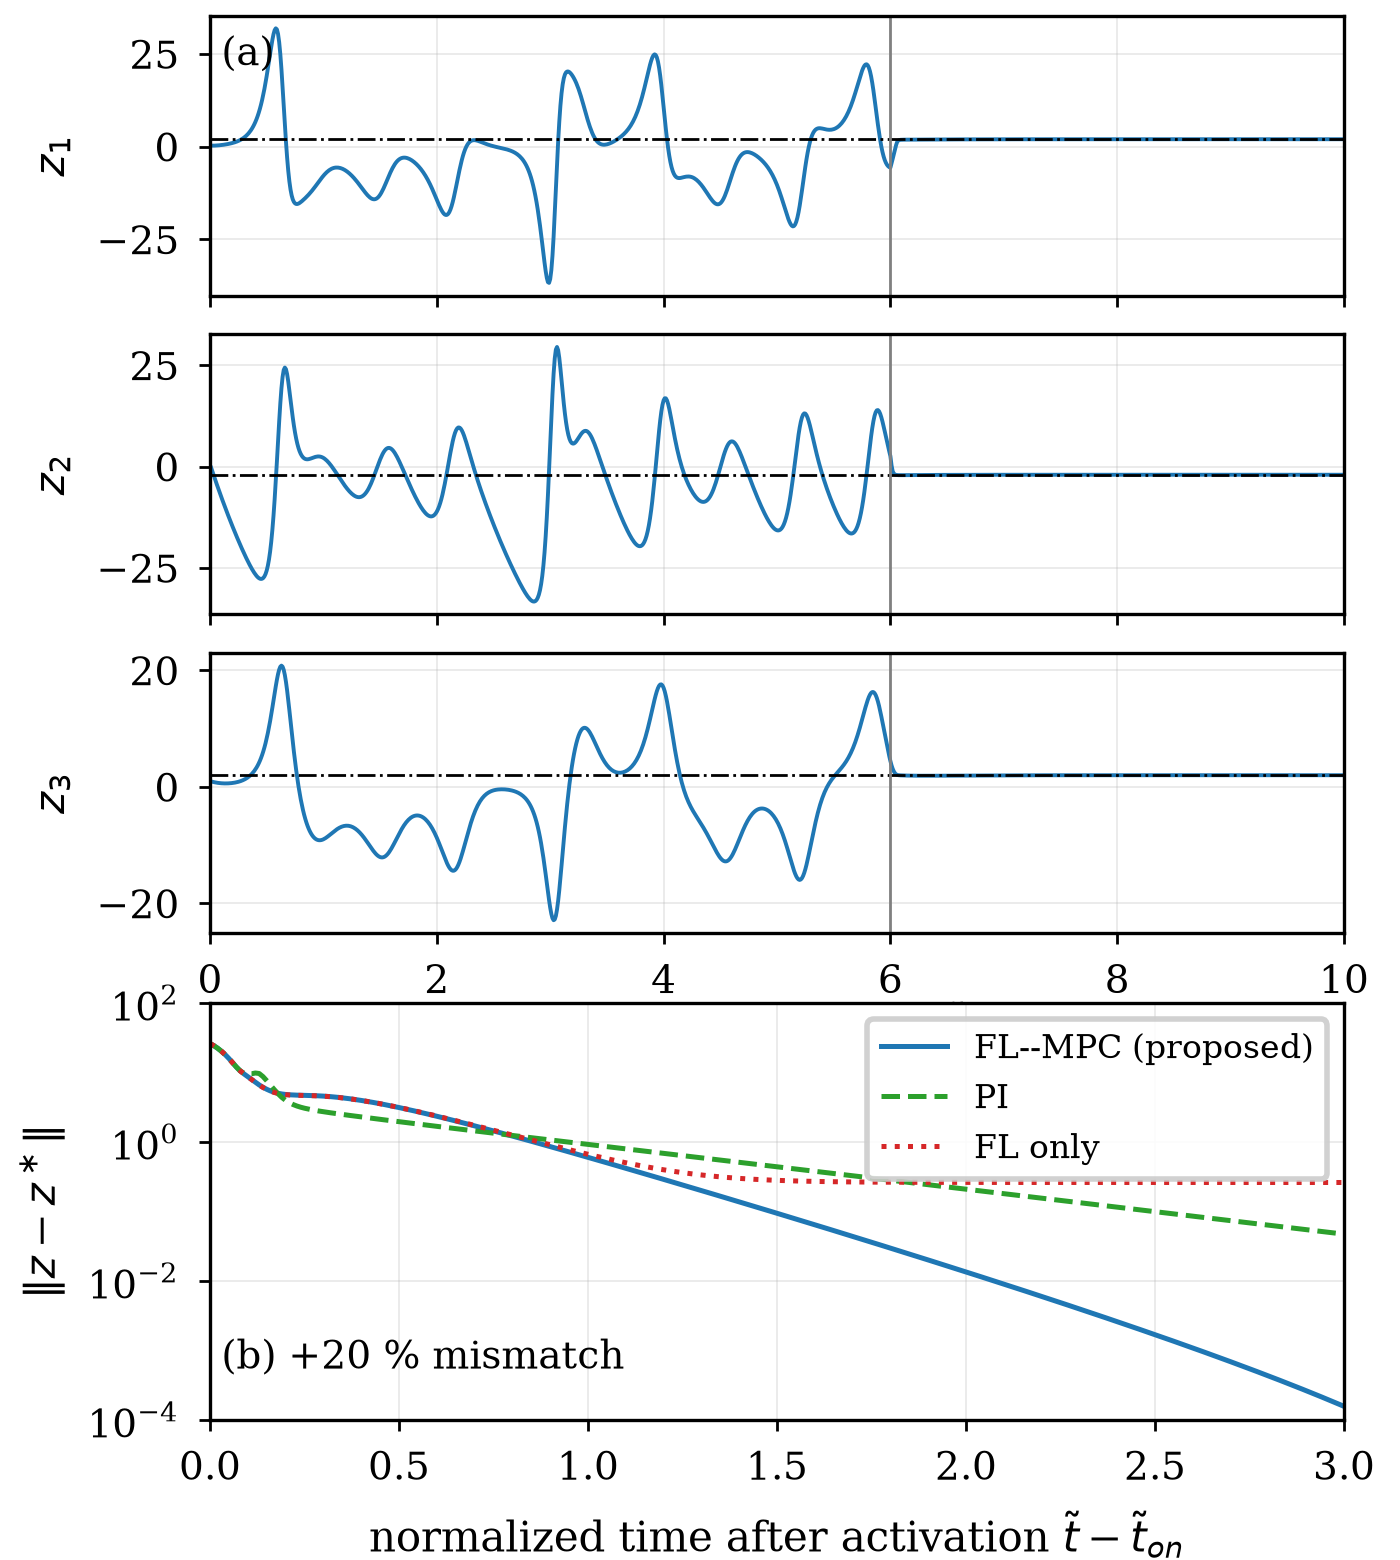
\includegraphics[width=0.48\textwidth]{fig4.png}}
\caption{Chaos suppression: (a) states of \eqref{eq5} with FL--MPC switched on at $\tilde t=6$ (dash-dot: target $z^\ast$); (b) error norm after activation with $+20\,\%$ plant mismatch.}
\label{fig4}
\end{figure}

\begin{table}[htbp]
\caption{Chaos Suppression Performance with $u_1,u_2$ Only (IAE of $\|z-z^\ast\|$, Settling Time $t_s$ to a 2\,\% Band, Final Error $e_f$; Normalized Time)}
\begin{center}
\begin{tabular}{|c|c|c|c|c|}
\hline
\textbf{Plant} & \textbf{Metric} & \textbf{FL--MPC} & \textbf{FL only} & \textbf{PI} \\
\hline
 & IAE & 0.42 & \textbf{0.41} & 0.72 \\
nominal & $t_s$ & 0.66 & \textbf{0.60} & 1.01 \\
 & $e_f$ & 0 & 0 & 0 \\
\hline
 & IAE & 2.18 & 4.51 & \textbf{1.98} \\
$-20\,\%$ & $t_s$ & \textbf{1.30} & -- & 2.13 \\
 & $e_f$ & 0 & 0.26 & 0 \\
\hline
 & IAE & \textbf{4.55} & 6.81 & 4.56 \\
$+20\,\%$ & $t_s$ & \textbf{1.57} & -- & 2.73 \\
 & $e_f$ & 0 & 0.26 & 0 \\
\hline
\end{tabular}
\label{tab2}
\end{center}
\end{table}

Fig.~\ref{fig4}(a) shows that the chaotic oscillations are suppressed as soon as the controller is activated, using only the rotor voltages, and the states settle at $z^\ast$. Table~\ref{tab2} and Fig.~\ref{fig4}(b) compare the three controllers. With an exact model, FL--MPC and FL only behave almost identically. Under mismatch, FL only keeps a steady-state error (0.26). PI and FL--MPC both converge without offset and have similar IAE, but FL--MPC settles 35--43\,\% faster (0.66--1.57 versus 1.01--2.73, i.e., 21--50~ms versus 32--88~ms with $\tau=32.1$~ms). All controllers reach the input limit during the first instants; the MPC accounts for it explicitly.

\subsection{MPPT Tracking of the 2-MW-Class DFIG}

The model \eqref{eq3} with Table~\ref{tab1} is driven by the wind of Fig.~\ref{fig2} for 30~s, with $T_s=1$~ms, $N=10$, $Q=\text{diag}(1,3)$ and $r=10^{-6}$ (errors scaled by 1~kA), and the outer speed loop uses $\lambda=10$~s$^{-1}$, $\lambda_I=25$~s$^{-2}$. The only inputs are the rotor voltages, limited to $|\Delta u_{dr}|,|\Delta u_{qr}|\le200$~V. Two mismatched plants are considered: M1 ($R_s,R_r$ $+20\,\%$, $L_m$ $-10\,\%$, $J$ $+20\,\%$) and M2 ($R_s,R_r$ $-20\,\%$, $L_m$ $+10\,\%$, $J$ $-20\,\%$), with the leakage inductances kept constant so that $L_s,L_r>L_m$ still holds.

\begin{figure}[htbp]
\centerline{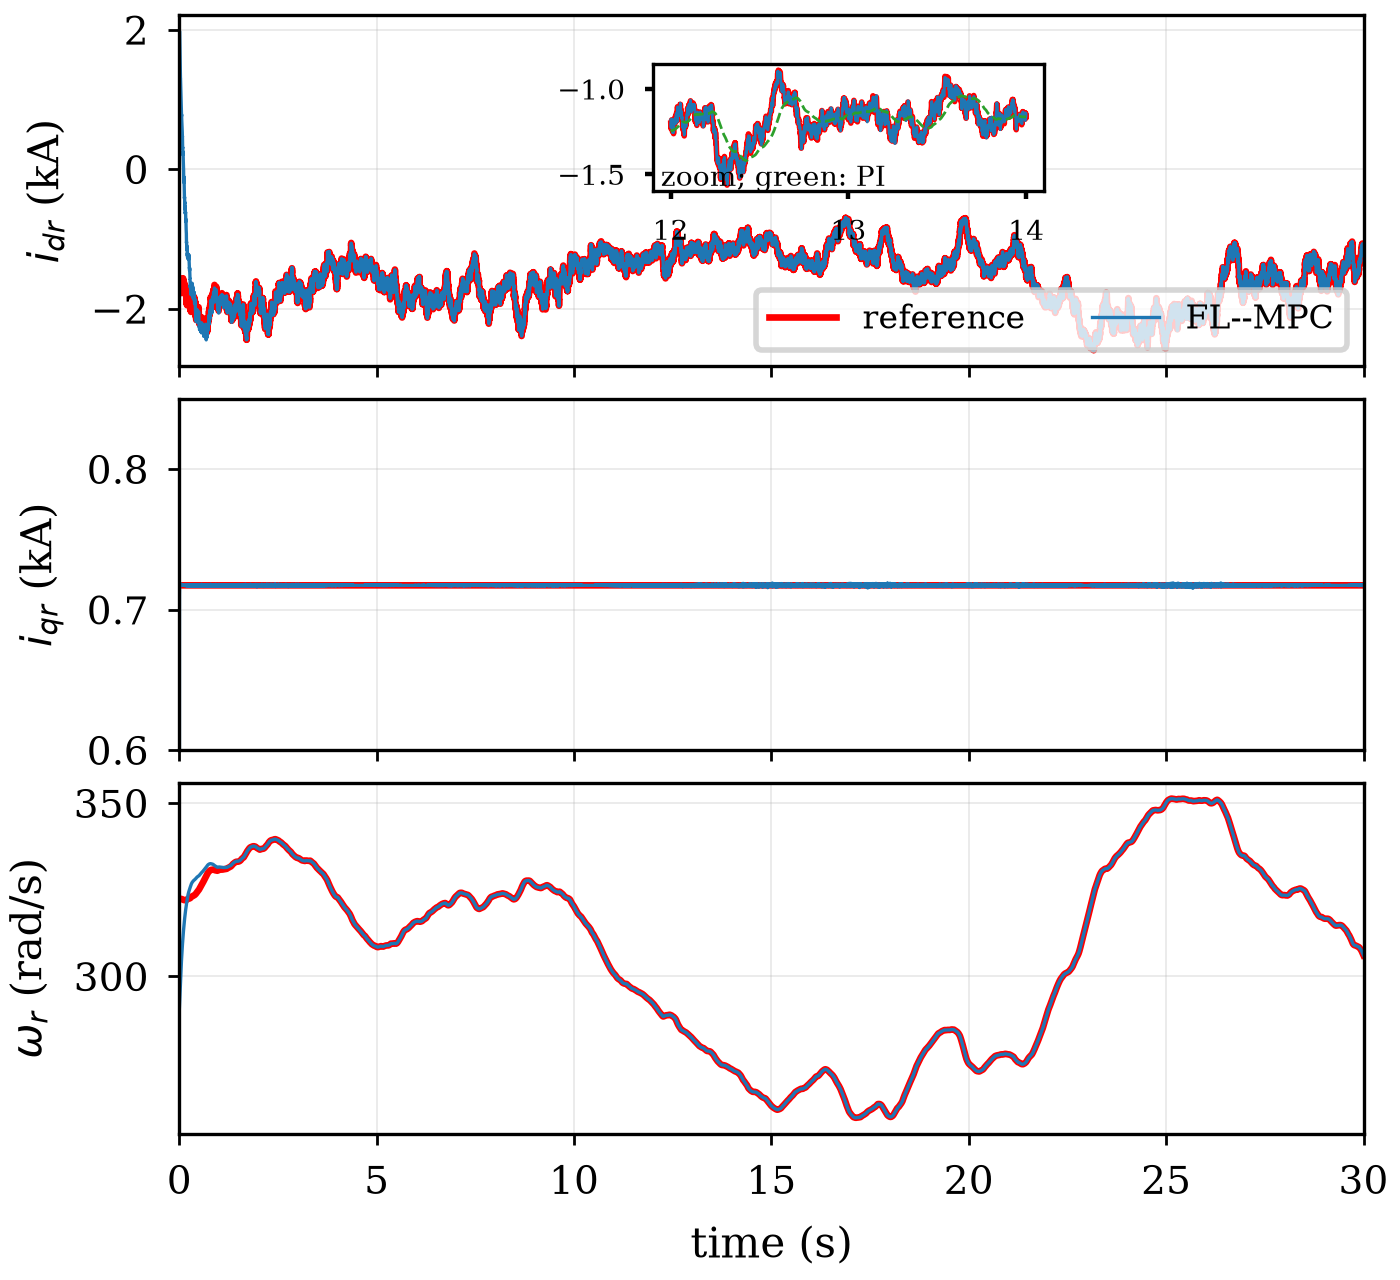
\includegraphics[width=0.48\textwidth]{fig5.png}}
\caption{Tracking of $i_{dr}$, $i_{qr}$ and $\omega_r$ with FL--MPC (nominal plant). Inset: zoom including PI.}
\label{fig5}
\end{figure}

\begin{figure}[htbp]
\centerline{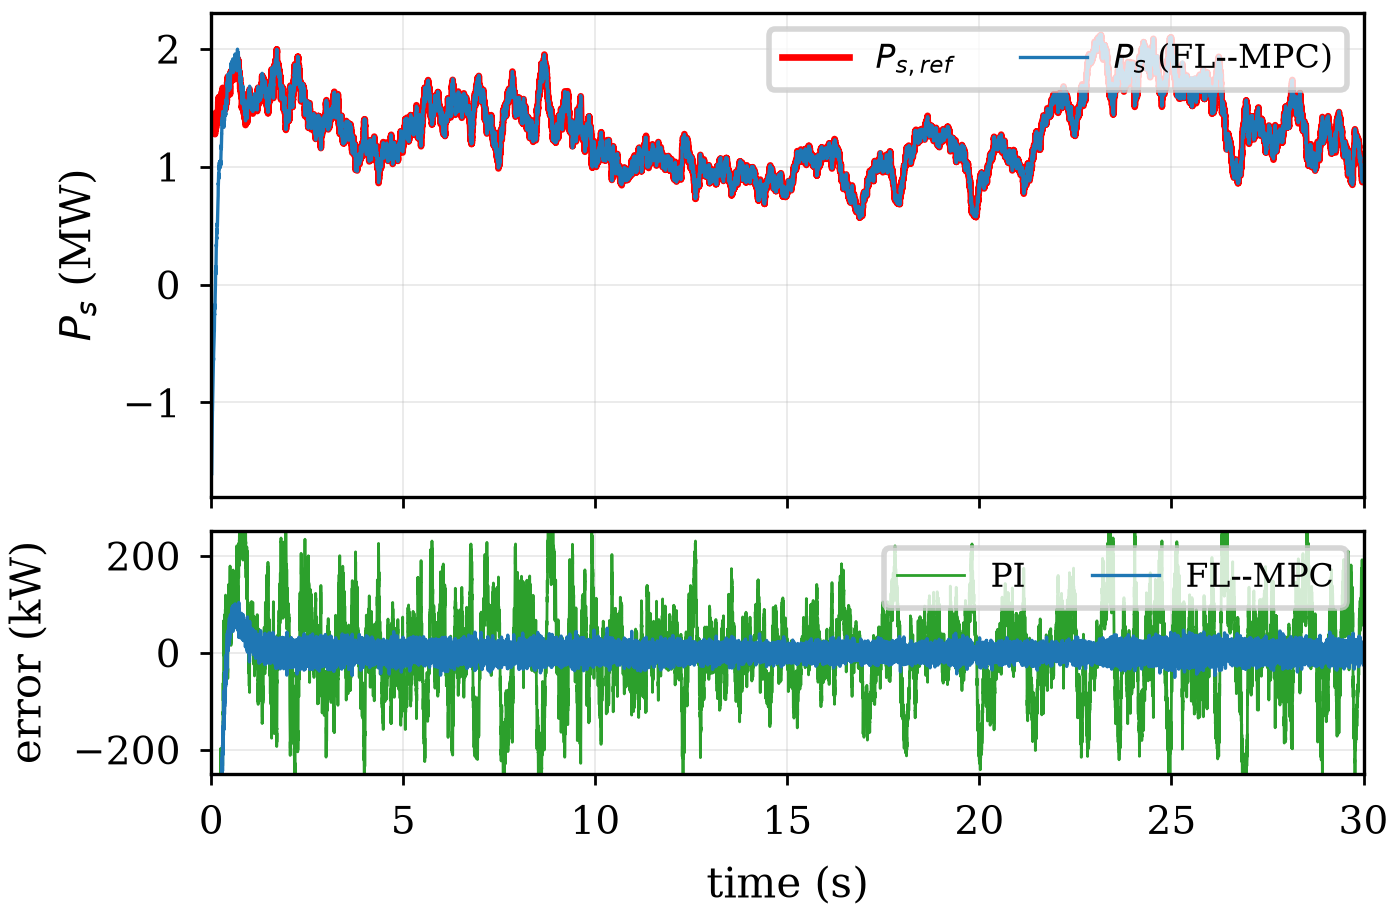
\includegraphics[width=0.48\textwidth]{fig6.png}}
\caption{Stator active power $P_s$ and MPPT reference $P_{s,ref}$ (FL--MPC), and power tracking errors of FL--MPC and PI.}
\label{fig6}
\end{figure}

\begin{table}[htbp]
\caption{MPPT Tracking Performance ($t\ge5$~s): RMS Errors of $P_s$ (\% of 2~MW), $i_{dr}$ (A) and $\omega_r$ (rad/s)}
\begin{center}
\begin{tabular}{|c|c|c|c|c|}
\hline
\textbf{Plant} & \textbf{RMSE} & \textbf{FL--MPC} & \textbf{FL only} & \textbf{PI} \\
\hline
 & $P_s$ & 0.59 & 0.59 & 4.61 \\
nominal & $i_{dr}$ & 14.3 & 14.3 & 112.9 \\
 & $\omega_r$ & 0.008 & 0.008 & 1.157 \\
\hline
 & $P_s$ & 1.65 & 1.65 & 5.02 \\
M1 & $i_{dr}$ & 40.5 & 40.5 & 122.8 \\
 & $\omega_r$ & 0.184 & 0.184 & 0.973 \\
\hline
 & $P_s$ & 1.65 & 1.65 & 4.59 \\
M2 & $i_{dr}$ & 40.3 & 40.3 & 112.4 \\
 & $\omega_r$ & 0.183 & 0.183 & 1.345 \\
\hline
\end{tabular}
\label{tab3}
\end{center}
\end{table}

Figs.~\ref{fig5} and \ref{fig6} show that the rotor currents, the speed and the stator power follow the MPPT references despite turbulence. The speed stays in the admissible slip range (0.82--1.12\,$\omega_s$), and $P_s$ varies between 0.57 and 2.1~MW. Starting from $0.9\,\omega_{r,ref}$, the speed enters the 2\,\% band in 0.13~s with FL--MPC, versus 0.77~s with PI. Table~\ref{tab3} shows that the speed RMS error of FL--MPC is 5--140 times lower than with PI, and its power RMS error is 0.59\,\% of rated power (nominal) and 1.65\,\% (mismatch), about three to eight times lower than with PI. Under mismatch, the larger $i_{dr}$ and $P_s$ errors with respect to the nominal MPPT reference mainly reflect that the torque current actually required changes with $J$ and $L_m$, while the speed is still tracked within 0.18~rad/s. For tracking, FL--MPC and FL only perform identically: the outer integral action compensates the mismatch, and the voltage limits are never reached by FL--MPC in this scenario (maximum 185~V). The main benefits of the MPC are therefore its explicit, stability-preserving treatment of constraints and its offset-free behaviour, which matter in large transients such as the recovery from chaos.

\section{Conclusion}

This paper revisited the nonlinear dynamics of a DFIG-based wind turbine with a physically consistent parameter set and explicit model constants. A dimensionless model shows that chaos, confirmed by a positive Lyapunov exponent and a bifurcation diagram, arises only under severely detuned damping and abnormal rotor excitation, i.e., as a fault scenario. A hybrid controller combining feedback linearization with a constrained MPC whose terminal ingredients are obtained from an LMI was proposed, with guaranteed nominal stability. The control acts only on the rotor voltages, the speed being governed through a cascaded torque-current loop. Simulations show chaos suppression without steady-state error under $\pm20\,\%$ mismatch with faster settling than PI, and MPPT tracking with speed and power errors several times lower than PI. Future work will address converter and grid dynamics, low-voltage ride-through, and experimental validation.

\section*{Conflict of Interest}
The authors declare that there are no conflicts of interest.

\balance
\begin{thebibliography}{00}
\bibitem{r1} International Energy Agency, \textit{World Energy Outlook 2024}. Paris, France: IEA, 2024. [Online]. Available: https://www.iea.org/reports/world-energy-outlook-2024
\bibitem{r2} International Renewable Energy Agency, \textit{Renewable Energy Statistics 2024}. Abu Dhabi, UAE: IRENA, Jul. 2024. [Online]. Available: https://www.irena.org/publications/2024/Jul/Renewable-energy-statistics-2024
\bibitem{r3} United Nations Environment Programme, \textit{Emissions Gap Report 2024}. Nairobi, Kenya: UNEP, 2024.
\bibitem{r4} Global Wind Energy Council, \textit{Global Wind Report 2024}. Brussels, Belgium: GWEC, Apr. 2024. [Online]. Available: https://gwec.net/global-wind-report-2024/
\bibitem{r5} Global Wind Energy Council, \textit{Global Wind Report 2025}. Brussels, Belgium: GWEC, Apr. 2025. [Online]. Available: https://www.gwec.net/reports/globalwindreport/2025
\bibitem{r6} International Energy Agency, \textit{Renewables 2024: Analysis and Forecast to 2030}. Paris, France: IEA, 2024. [Online]. Available: https://www.iea.org/reports/renewables-2024
\bibitem{r7} R. Pena, J. C. Clare, and G. M. Asher, ``Doubly fed induction generator using back-to-back PWM converters and its application to variable-speed wind-energy generation,'' \textit{IEE Proc.---Electr. Power Appl.}, vol. 143, no. 3, pp. 231--241, May 1996.
\bibitem{r8} S. M\"uller, M. Deicke, and R. W. De Doncker, ``Doubly fed induction generator systems for wind turbines,'' \textit{IEEE Ind. Appl. Mag.}, vol. 8, no. 3, pp. 26--33, May/Jun. 2002.
\bibitem{r9} S. Heier, \textit{Grid Integration of Wind Energy: Onshore and Offshore Conversion Systems}, 3rd ed. Chichester, U.K.: Wiley, 2014.
\bibitem{r10} M. G. Sim\~oes and F. A. Farret, \textit{Modeling and Analysis with Induction Generators}, 3rd ed. Boca Raton, FL, USA: CRC Press, 2015.
\bibitem{r11} A. A. Chhipa \textit{et al.}, ``Modeling and control strategy of wind energy conversion system with grid-connected doubly-fed induction generator,'' \textit{Energies}, vol. 15, no. 18, Art. no. 6694, 2022, doi: 10.3390/en15186694.
\bibitem{r12} L. Xu and Y. Wang, ``Dynamic modeling and control of DFIG-based wind turbines under unbalanced network conditions,'' \textit{IEEE Trans. Power Syst.}, vol. 22, no. 1, pp. 314--323, Feb. 2007, doi: 10.1109/TPWRS.2006.889113.
\bibitem{r13} A. Tapia, G. Tapia, J. X. Ostolaza, and J. R. S\'aenz, ``Modeling and control of a wind turbine driven doubly fed induction generator,'' \textit{IEEE Trans. Energy Convers.}, vol. 18, no. 2, pp. 194--204, Jun. 2003, doi: 10.1109/TEC.2003.811727.
\bibitem{r14} Y. Lei, A. Mullane, G. Lightbody, and R. Yacamini, ``Modeling of the wind turbine with a doubly fed induction generator for grid integration studies,'' \textit{IEEE Trans. Energy Convers.}, vol. 21, no. 1, pp. 257--264, Mar. 2006, doi: 10.1109/TEC.2005.847958.
\bibitem{r15} H. Nian, Y. Song, P. Zhou, and Y. He, ``Improved direct power control of a wind turbine driven doubly fed induction generator during transient grid voltage unbalance,'' \textit{IEEE Trans. Energy Convers.}, vol. 26, no. 3, pp. 976--986, Sep. 2011, doi: 10.1109/TEC.2011.2158436.
\bibitem{r16} D. Xiang, L. Ran, P. J. Tavner, and S. Yang, ``Control of a doubly fed induction generator in a wind turbine during grid fault ride-through,'' \textit{IEEE Trans. Energy Convers.}, vol. 21, no. 3, pp. 652--662, Sep. 2006.
\bibitem{r17} J. Morren and S. W. H. de Haan, ``Ridethrough of wind turbines with doubly-fed induction generator during a voltage dip,'' \textit{IEEE Trans. Energy Convers.}, vol. 20, no. 2, pp. 435--441, Jun. 2005, doi: 10.1109/TEC.2005.845526.
\bibitem{r18} M. Rahimi and M. Parniani, ``Efficient control scheme of wind turbines with doubly fed induction generators for low-voltage ride-through capability enhancement,'' \textit{IET Renew. Power Gener.}, vol. 4, no. 3, pp. 242--252, May 2010, doi: 10.1049/iet-rpg.2009.0072.
\bibitem{r19} M. Tsili and S. Papathanassiou, ``A review of grid code technical requirements for wind farms,'' \textit{IET Renew. Power Gener.}, vol. 3, no. 3, pp. 308--332, Sep. 2009, doi: 10.1049/iet-rpg.2008.0070.
\bibitem{r20} M. Rahimi and M. Parniani, ``Dynamic behavior and transient stability analysis of fixed speed wind turbines,'' \textit{Renew. Energy}, vol. 34, no. 12, pp. 2613--2624, Dec. 2009, doi: 10.1016/j.renene.2009.06.019.
\bibitem{r21} Y. Yu, Z. Mi, and X. Liu, ``Analysis of chaos in doubly fed induction generator and sliding mode control of chaos synchronization,'' \textit{Acta Phys. Sin.}, vol. 60, no. 7, Art. no. 070509, 2011, doi: 10.7498/aps.60.070509.
\bibitem{r22} C. N. Van, N. T. Hai, and N. P. Quang, ``Chaos control of doubly-fed induction generator via delayed feedback control,'' \textit{Eng. Technol. Appl. Sci. Res.}, vol. 13, no. 2, pp. 10588--10594, Apr. 2023, doi: 10.48084/etasr.5812.
\bibitem{r23} P. A. Meehan, ``Prediction and suppression of chaos following flutter in wind turbines,'' \textit{Nonlinear Dyn.}, vol. 111, pp. 22153--22176, 2023, doi: 10.1007/s11071-023-08841-9.
\bibitem{r24} H. Ren and D. Liu, ``Nonlinear feedback control of chaos in permanent magnet synchronous motor,'' \textit{IEEE Trans. Circuits Syst. II, Exp. Briefs}, vol. 53, no. 1, pp. 45--50, Jan. 2006.
\bibitem{r25} M. Messadi and A. Mellit, ``Control of chaos in an induction motor system with LMI predictive control and experimental circuit validation,'' \textit{Chaos, Solitons Fractals}, vol. 97, pp. 51--58, 2017.
\bibitem{r26} G. Chen, ``A simple adaptive feedback control method for chaos and hyper-chaos control,'' \textit{Appl. Math. Comput.}, vol. 217, no. 17, pp. 7258--7264, 2011.
\bibitem{r27} H. Takhi, K. Kemih, L. Moysis, \textit{et al.}, ``Passivity based control and synchronization of perturbed uncertain chaotic systems and their microcontroller implementation,'' \textit{Int. J. Dyn. Control}, vol. 8, no. 3, pp. 973--990, 2020, doi: 10.1007/s40435-020-00618-x.
\bibitem{r28} A. Boukabou, A. Chebbah, and N. Mansouri, ``Predictive control of continuous chaotic systems,'' \textit{Int. J. Bifurcation Chaos}, vol. 18, no. 2, pp. 587--592, 2008, doi: 10.1142/S0218127408020501.
\bibitem{r29} A. Senouci and A. Boukabou, ``Predictive control and synchronization of chaotic and hyperchaotic systems based on a T--S fuzzy model,'' \textit{Math. Comput. Simul.}, vol. 105, pp. 62--78, 2014.
\bibitem{r30} M. Messadi and A. Mellit, ``Predictive control of a chaotic permanent magnet synchronous generator in a wind turbine system,'' \textit{Chin. Phys. B}, vol. 24, no. 1, Art. no. 010502, 2015.
\bibitem{r31} H. Takhi, L. Moysis, N. Machkour, C. Volos, K. Kemih, and M. Ghanes, ``Predictive control and synchronization of uncertain perturbed chaotic permanent-magnet synchronous generator and its microcontroller implementation,'' \textit{Eur. Phys. J. Spec. Top.}, vol. 231, no. 3, pp. 443--451, 2022, doi: 10.1140/epjs/s11734-021-00422-4.
\bibitem{r32} A. Mechter, K. Kemih, and M. Ghanes, ``Sliding mode control of a wind turbine with exponential reaching law,'' \textit{Acta Polytech. Hung.}, vol. 12, no. 3, pp. 167--183, 2015.
\bibitem{r33} I. Bouguettah, M. Messadi, K. Kemih, A. T. Azar, and A. R. Mahlous, ``Adaptive passive fault tolerant control of DFIG-based wind turbine using a self-tuning fractional integral sliding mode control,'' \textit{Front. Energy Res.}, vol. 12, Art. no. 1429877, 2024, doi: 10.3389/fenrg.2024.1429877.
\bibitem{r34} M. Messadi, K. Kemih, and H. Hamiche, ``A new secure communications scheme based on synchronization of hybrid chaotic system,'' \textit{Chaos Theory Appl.}, vol. 5, no. 3, pp. 160--166, 2023, doi: 10.51537/chaos.1276714.
\bibitem{r35} P. Jiang, T. Zhang, J. Geng, P. Wang, and L. Fu, ``An MPPT strategy for wind turbines combining feedback linearization and model predictive control,'' \textit{Energies}, vol. 16, no. 10, Art. no. 4244, 2023, doi: 10.3390/en16104244.
\bibitem{r36} S. Regani, M. Messadi, and K. Kemih, ``Modeling and nonlinear dynamic analysis of a DFIG-based wind turbine system,'' submitted for publication.
\bibitem{r37} A. Mechter, K. Kemih, and M. Ghanes, ``Backstepping control of a wind turbine for low wind speeds,'' \textit{Nonlinear Dyn.}, vol. 84, no. 4, pp. 2435--2445, 2016, doi: 10.1007/s11071-016-2655-y.
\bibitem{r38} A. Wolf, J. B. Swift, H. L. Swinney, and J. A. Vastano, ``Determining Lyapunov exponents from a time series,'' \textit{Physica D}, vol. 16, no. 3, pp. 285--317, 1985.
\bibitem{r39} D. Q. Mayne, J. B. Rawlings, C. V. Rao, and P. O. M. Scokaert, ``Constrained model predictive control: Stability and optimality,'' \textit{Automatica}, vol. 36, no. 6, pp. 789--814, 2000, doi: 10.1016/S0005-1098(99)00214-9.
\bibitem{r40} M. V. Kothare, V. Balakrishnan, and M. Morari, ``Robust constrained model predictive control using linear matrix inequalities,'' \textit{Automatica}, vol. 32, no. 10, pp. 1361--1379, 1996.
\end{thebibliography}

\end{document}
